\chapter{Development environment design}\label{chap:editor}
This chapter provides a design for Dual's development environment. This is not a formal specification. I try to provide an idea of how I imagine a good development environment should look like to maximize usability and be appealing to experienced as well as semi-experienced programmers.

These are general guidelines that may be applied to improve existing visual programming language systems in terms of usability.

A proof-of-concept prototype implementation that, to a degree, conforms to the design outlined here, is described in Chapter \ref{chap:impl}. In that implementation I focus on the critical features that are necessary to meet the goals of this thesis.

\section{Overview}
The overall design tries to merge features of modern code editors, such as Brackets\cite{brackets_site}, Visual Studio Code\cite{vscode_site} or Atom\cite{atom_site} with visual programming language editors, such as the Blueprint Editor from Unreal Engine 4\cite{blueprint_editor}.

The environment is intended to work online, similarly to \acrlong{ide}s such as Codeanywhere\cite{codeanywhere_website} or Cloud9\cite{c9_website}. It should also work as offline, like Scratch's offline editor\cite{scratch_offline}.

\section{Design goals}
I set the following general goals that the designed development environment must meet:
\begin{itemize}
\item In terms of usability, it should be easily usable with minimal effort from the user to install it or set it up.
\item The user interface and its idioms and metaphors\cite{ui_idioms} should be familiar for an experienced user and easy to learn for an inexperienced one.
\item The editor should support the text and visual representation.
% and should provide an interface to add new representations.
\end{itemize}

\section{Requirements}
In order to meet the above goals, I set down the design requirements outlined in this section.

\subsection{Usability}
The environment should be a web application. It should have minimal external dependencies.

It should be separated into the following components:
\begin{itemize}
\item A project manager, which should be capable of managing local as well as remote projects. The environment identifies projects by paths, which obviates the need for project files.

For example, if user selects a path on her local file system, such as \texttt{~/projects/my-project}, it will be registered as the most recently opened project and opened in the editor. All files contained in the \texttt{my-project} folder would be a part of the project.

This is an idiom used in modern code editors, such as Brackets or Visual Studio Code. However, project files could be optional.

\item A code editor, which itself consists of two parts:
    \begin{itemize}
    \item A text editor with syntax highlighting, auto-completion, auto-indentation, etc. for Dual. The text editor should conform to the design outlined in Section \ref{sec:est}.
    \item A visual editor able to manipulate a visual representation of the EST  with autostructuring. It should also conform to the design outlined in Section \ref{sec:est}.
    \end{itemize}
\end{itemize}


\subsection{User interface}
The general layout of the editor should conform to universally accepted (\textit{de facto}) standards where possible. As illustrated in Figures \ref{fig:vs_code_ss}, \ref{fig:atom_ss} and \ref{fig:brackets_ss}, different code edtiors feature a very similar layout. Below I aim to enumerate its general features.

The layout of Dual's environment should include the following:
\begin{itemize}
\item A title bar, which contains the name of the file that is currently being edited (focused), a path to the file and the name of the editor.
\item A menu bar at the very top of the window screen, which contains menus such as File, Edit, View, Help, each with appropriate options and submenus.
\item A left panel with a tree view of all the files that belong to the currently open project. 
\item Next to the left panel, a main area, where the contents of the currently open file are displayed. There may be a split view functionality, where a few files can be displayed at once next to each other. There also may be a tab bar above a file's contents that contains buttons that allow the user to quickly switch between several open files.
\item A bottom panel that can contain an interactive console, similar to the JavaScript console in web browsers. The panel may also display various status information.
\item A status bar at the bottom of the screen. It may display short information about current position in a file, text encoding or indentation size.
\item A text input that is an interface for a flexible global search facility, which can search through all editor options and menus, as well as the library of available programming language constructs: all primitives, basic functions and macros as well as all user-defined functions and macros. The search functionality should be available at all times. It should appear at the top of the screen and may be toggleable.
\end{itemize}

\begin{figure}[h!]
\centering 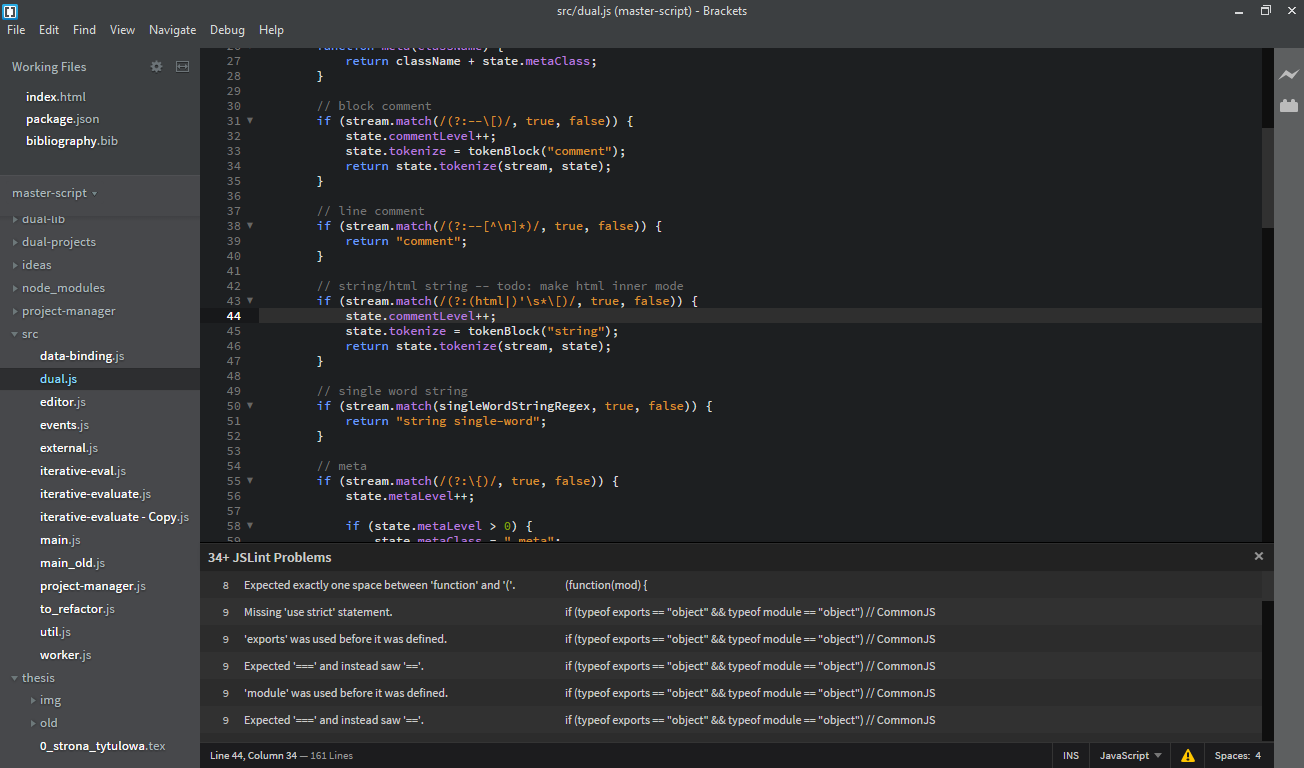
\includegraphics[width=0.9\textwidth]{brackets_ss}
\caption{
    A screenshot from the Brackets editor
}
\label{fig:brackets_ss}
\end{figure}

\begin{figure}[h!]
\centering 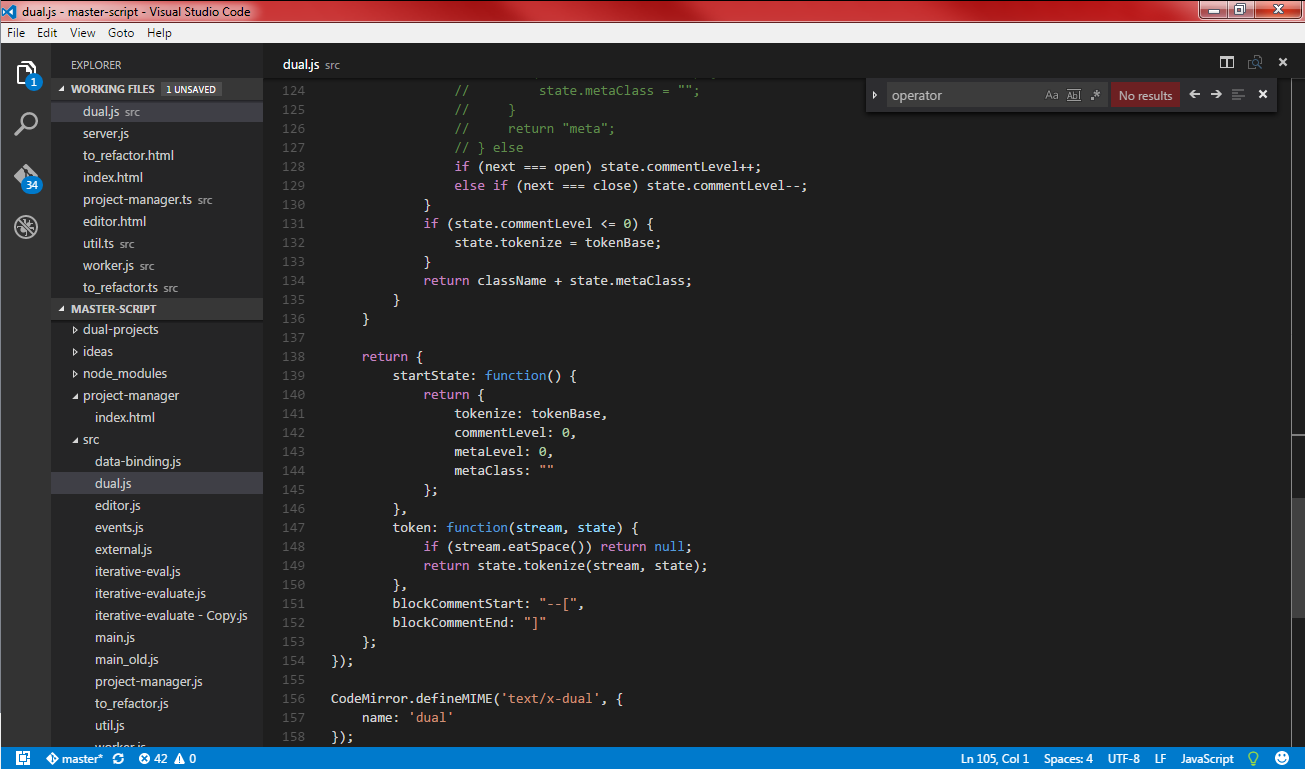
\includegraphics[width=0.9\textwidth]{vs_code_ss}
\caption{
    A screenshot from the Visual Studio Code editor
}
\label{fig:vs_code_ss}
\end{figure}

\begin{figure}[h!]
\centering 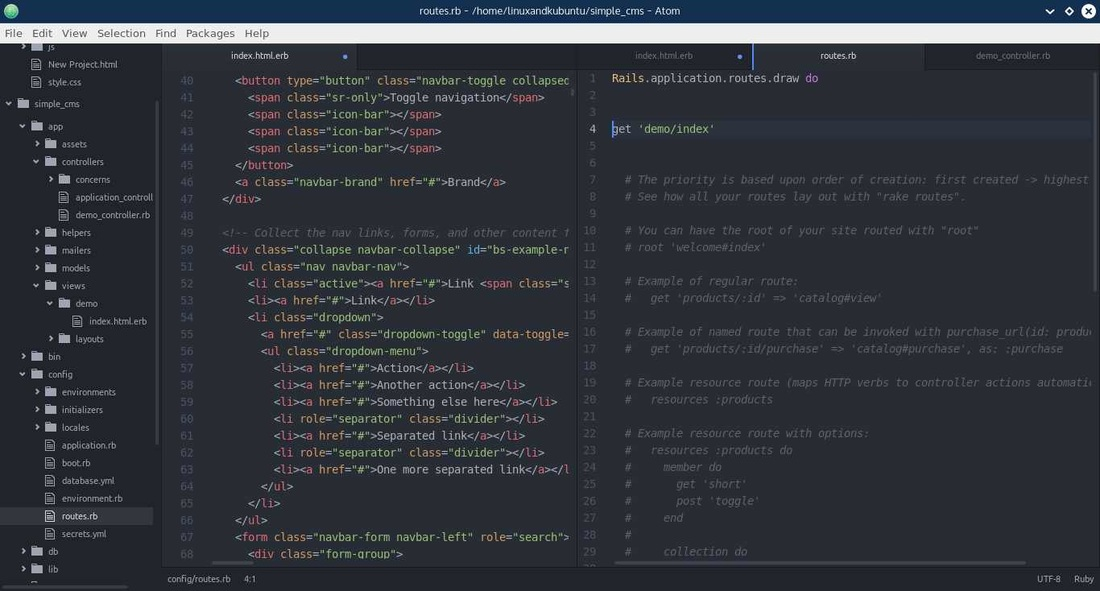
\includegraphics[width=0.9\textwidth]{atom_ss}
\caption{
    A screenshot from the Atom editor
}
\label{fig:atom_ss}
\end{figure}


\section{Text editor}
The text editor should have all the standard capabilities of modern code editors, like the ones outlined in Section \ref{sub:text_editors}:
\begin{itemize}
	\item Auto-indentation.
	\item Syntax highlighting.
	\item Code folding. Any code between a matching pair of brackets should be collapsible.
	\item Code navigation. Any identifier or module path in the source code should be a link to an appropriate declaration or definition, if such is available.
	\item Context-sensitive auto-completion. This includes automatic pairing of brackets and correction of typing errors.
    \item Find and replace functionalities with support for regular expressions.
    \item The source text should be processed by the editor as a two dimensional grid of characters, with each row (line) and column numbered. Any rectangular area in this grid should be selectable.
    \item Related to the above: editing of multiple lines in parallel. If an area is selected that spans multiple rows, each row has its own text cursor.
\end{itemize}

All of the above features should be integrated with the language and make use of its parser and the syntax tree generated by it.

\section{Visual editor and its editor}
In order to address some of the most common criticisms of VPLs, outlined in Section \ref{sub:vpl_crit} I set the following general design requirements for the visual representation:
\begin{itemize}
\item It should combine the familiar appearance of the ``line-connected block-based'' VPLs with the structure of ``snap-together block-based'' VPLs (see Section \ref{sec:vpls}). The former family is exemplified by the Blueprints Visual Scripting system of Unreal Engine 4\cite{blueprint} and the latter by MIT Scratch\cite{scratch, scratch_wikipedia}.
\item It should be no harder to use than the text representation. Ideally a visual editor should add useful capabilities, without taking away these provided by text editors.
\item Its appearance should be fully customizable.
\end{itemize}

Moreover, Dual's visual representation should satisfy all the requirements outlined in \ref{sec:est}:
\begin{itemize}
\item It should be fully mappable to the EST. There should be a distinguishable and manipulable visual element for every EST node. Such an element should contain a reference to the node (and vice versa).

\item There should be ways to perform the following actions with the visual editor:
    \begin{itemize}
    \item Insert new nodes into EST.
    \item Remove existing nodes from the EST.
    \item Modify existing nodes in the EST.
    \item Replace existing nodes and subtrees in the EST.
    \item Move nodes and subtrees to different locations in the EST.
    \item Select and manipulate multiple arbitrary nodes and subtrees in the EST.
    \end{itemize}
    
In short, the visual editor should provide ways to perform the same abstract operations on the EST that are possible when editing text and possibly more.
\end{itemize}

Some operations on raw text should also be reflected in the visual representation. For example the Find option. Searching through text should highlight the visual elements that correspond to the EST nodes that are connected to the text that contains the searched phrase. Regular expression based searching should also be possible. Replacing text with the Replace option should be reflected in the visual representation.

There should be a possibility to temporarily disable a representation by disconnecting it from the EST. Any changes made to other representations will then not be propagated to this representation. A disabled representation should become read-only until it is enabled. When it is enabled it should be updated to reflect the current state of the EST. At least one representation must be enabled at all times.

There should be a context-sensitive auto-completion feature and an easily accessible library of functions and primitives with documentation. User-defined functions should be added to the library and auto-completion database upon definition and removed from it when they are removed from the source code.

The library could look similarly to the one in Scratch, where the user can select puzzle pieces from several categories (Figure \ref{fig:scratch2}). The categories should be the names of modules, where each function is defined. Similarly, submodules should have their respective subcategories.

The auto-completion context menu could resemble the one from the UE4's Blueprint editor (Figure \ref{fig:blu_context}). If there is many auto-completion possibilities, they should be presented as a tree, with categories from the library as root nodes.

\begin{figure}[h!]
\centering 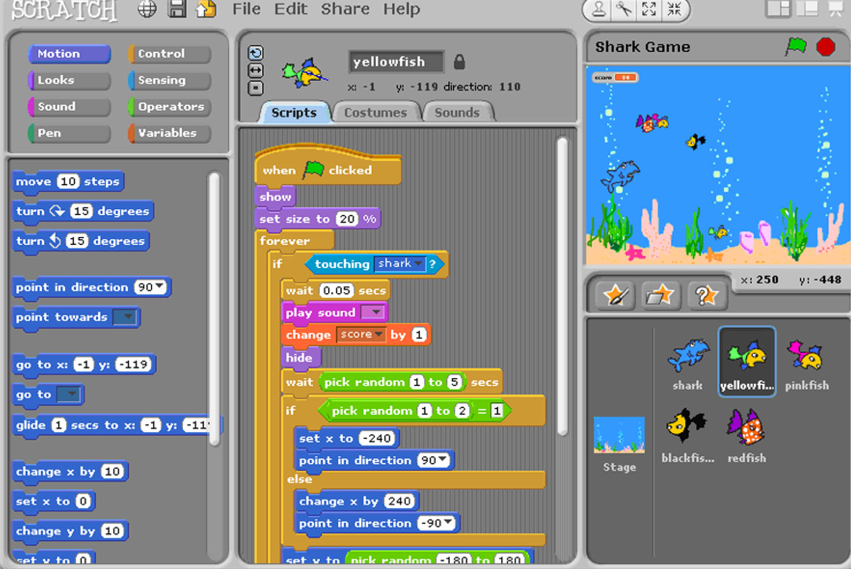
\includegraphics[width=0.9\textwidth]{scratch}
\caption{
    MIT Scratch programming language editor;
    the left panel contains a library of language constructs. These are ordered into categories (selectable with buttons at the top of the panel);
    screenshot from\protect\cite{fig_scratch}
}
\label{fig:scratch2}
\end{figure}

\begin{figure}[h!]
\centering 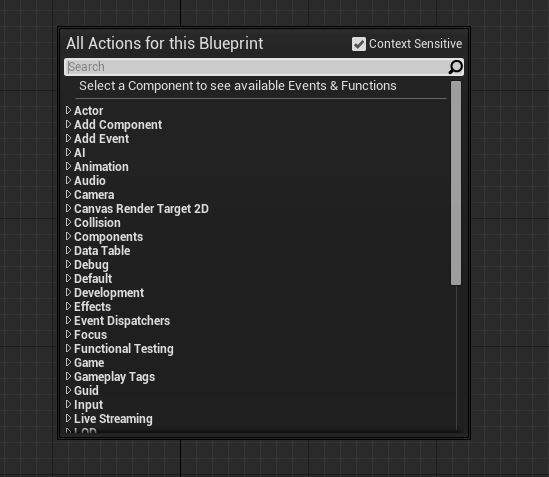
\includegraphics[width=0.9\textwidth]{blu_context}
\caption{
    The context menu from the UE4's Blueprints editor;
    each item is a category, which can be expanded by clicking on it into subcategories, which eventually lead to individual nodes. Clicking on a node name inserts it into the program;
    screenshot from\protect\cite{fig_blu_context}
}
\label{fig:blu_context}
\end{figure}

\subsection{The design process}
Figures \ref{fig:designs_01234}, \ref{fig:design_3}, and \ref{fig:design_4} show mock-ups that were produced when designing the visual representation.

The colored squares with letters inside are place-holders for icons. The user should be able to click on those icons and fold the blocks into a more compact form, hiding the names and excessive text. This may be done on the level of individual blocks, whole subtrees or the entire program -- similar to code folding in text editors. This allows to have a big picture and general relationships between nodes always visible and at the same time gives an ability to focus on the details of the part at hand.

The design contains the following visual elements:
\begin{itemize}
	\item Rectangular blocks, which represent expressions or individual nodes of the \acrshort{est}. Those in turn consist of:
	\begin{itemize}
		\item A header, which contains an icon and the name of the expression's operator. Next to the header a documentation comment may be displayed.
		\item Slots, which are the numbers or names of the arguments followed by an icon. Below these documentation comments may be displayed.
		\item Additional buttons, which may be used for example to add more slots to variadic expressions.
	\end{itemize}
	\item Connections between slots and blocks, which could also contain
          some useful annotations. The proposed design places type annotations
          there. These consist of the name of the type followed by an icon that
          represents this type. Connections actually have two parts: one
          extending from a slot, which in this case would contain the argument's
          type annotation, and one extending from a block header, which would
          contain a type annotation of the expression's return value.
\end{itemize}

Icons are a way to minimize the use of text to represent different entities. The text below the slots could be documentation comments associated with the
given argument. Their visibility could be toggleable through clicking on them,
on an individual or global basis, similarly to icons.

We can observe that there's a need to manipulate or set visual properties of
individual objects, clusters of objects/subtrees as well as the entire program
tree.

The text representation is very compact, which often is an advantage. This
advantage can be maintained by the visual representation by making all the
additional information optional. The user should have easy way of configuring
whether or not and what informations should be displayed. By folding some
textual elements into icons the visual representation could actually be made
more compact than the text form.

The visual form allows us to provide much more information about different
elements of the program. Spatially relate this information with these elements
through blocks and connections. Relate expressions with other expressions
through connections, which can also carry additional information.

\begin{figure}[h!]
\centering 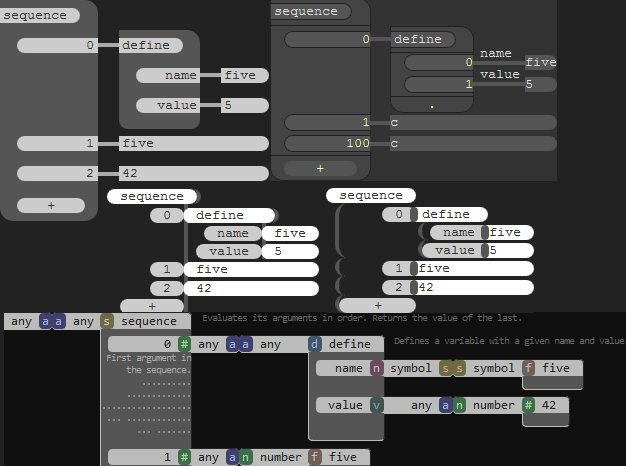
\includegraphics[width=0.9\textwidth]{designs_01234}
\caption{}
\label{fig:designs_01234}
\end{figure}

\begin{figure}[h!]
\centering 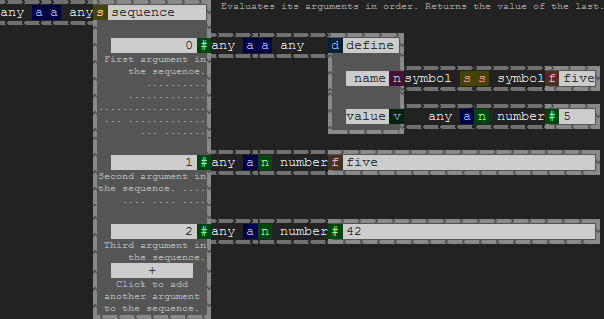
\includegraphics[width=0.9\textwidth]{design_3}
\caption{This design has the interesting property of visually illustrating the
  program flow with arrows.}
\label{fig:design_3}
\end{figure}

\begin{figure}[h!]
\centering 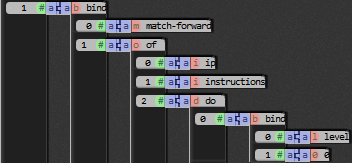
\includegraphics[width=0.9\textwidth]{design_4}
\caption{}
\label{fig:design_4}
\end{figure}

\section{Debugging}
Both, the text and the visual editor should provide an interface for debugging programs. This entails the abilities to:
\begin{itemize}
\item Set breakpoints on individual lines of code (applicable only to the text editor).
\item Set breakpoints on individual expressions (applicable to both).
\item Pause program execution and step over, in and out of individual expressions.
\item Inspect program state. It should be possible to easily access the values of individual expressions and possibly change them.
\item Signal errors in a specific and readable manner.
\end{itemize}

Other features that aid debugging could also be useful. For example:
\begin{itemize}
\item The ability to record program execution and rewind it, inspecting individual steps.
\item Support for exceptions.
\item Support for remote debugging.
\item Profiling facilities.
\end{itemize}

\section{Additional features}
The editor should also provide the following additional features:
\begin{itemize}
\item Integration with version control systems and services that provide it, such as GitHub.
\item Integration with text comparison and diff tools.
\item Integration with linting tools. 
\item An \acrlong{api} for plugin creation.
\item ``Intelligent'' mechanisms that display contextual hints and suggestions.
\end{itemize}
 